\begin{figure}[htpb]
	\centering\capstart{}
	\subfloat[\(\mesh{S_{1}},\ \mu_{1}=1.00\)]
	{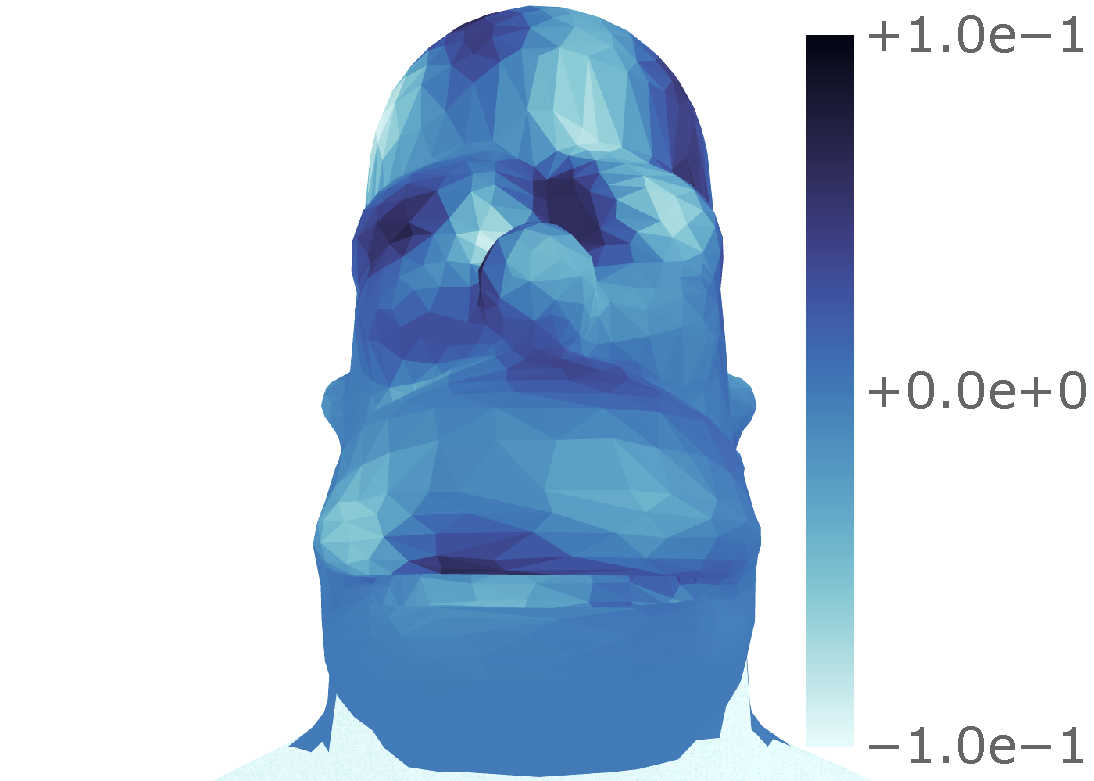
\includegraphics[trim={101 0 3 3},clip,width=.33\textwidth]{slepian_homer_rank0_lam1-000000e00_zoom.pdf}} % chktex 8
	\hfill
	\subfloat[\(\mesh{S_{10}},\ \mu_{10}=1.00\)]
	{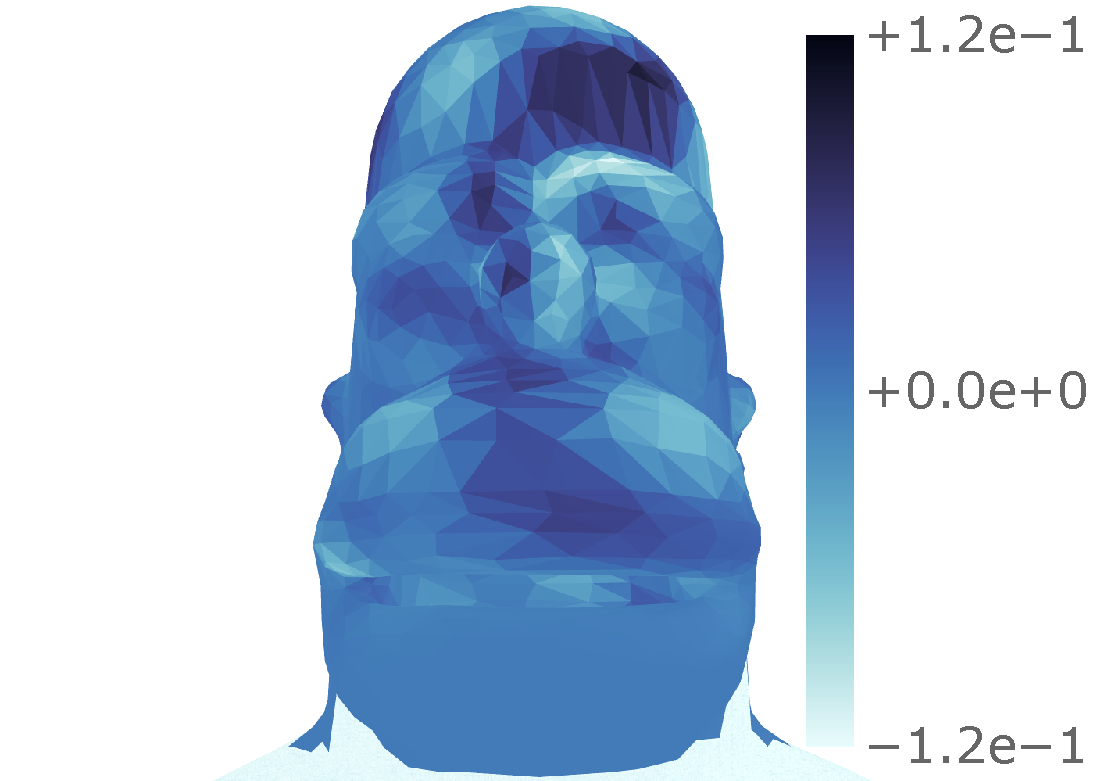
\includegraphics[trim={101 0 3 3},clip,width=.33\textwidth]{slepian_homer_rank9_lam1-000000e00_zoom.pdf}} % chktex 8
	\hfill
	\subfloat[\(\mesh{S_{25}},\ \mu_{25}=1.00\)]
	{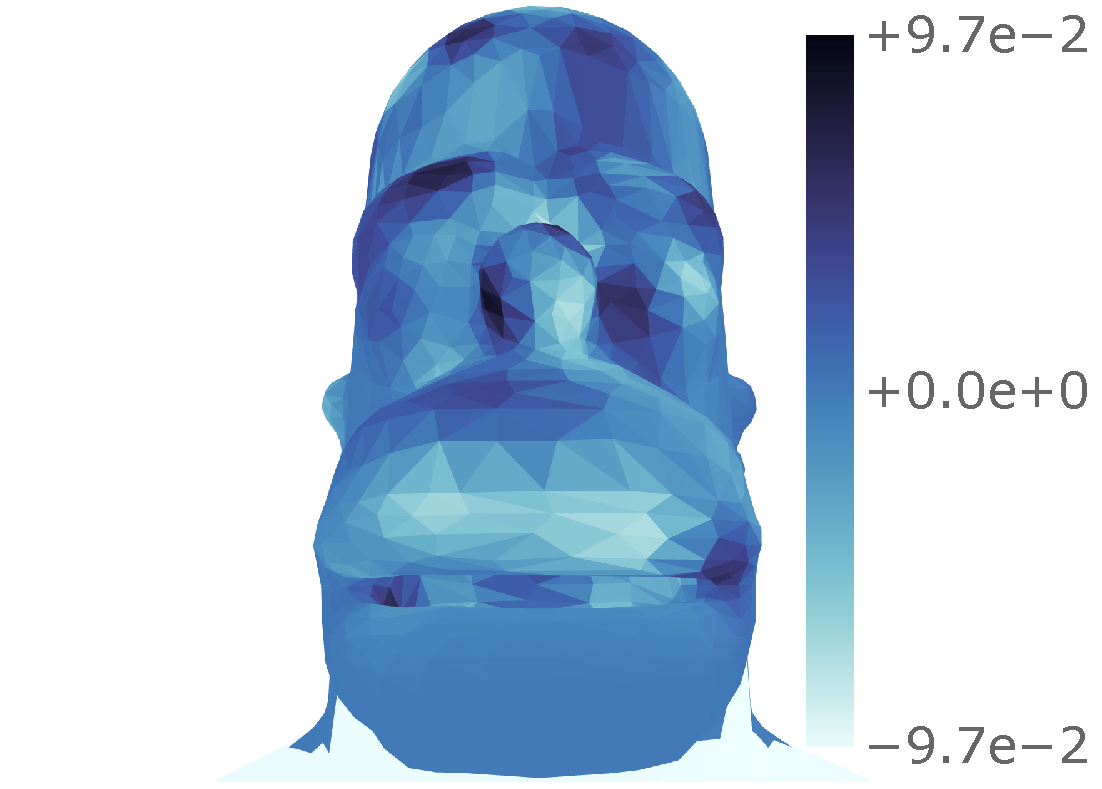
\includegraphics[trim={101 0 3 3},clip,width=.33\textwidth]{slepian_homer_rank24_lam1-000000e00_zoom.pdf}} % chktex 8
	\newline
	\subfloat[\(\mesh{S_{50}},\ \mu_{50}=1.00\)]
	{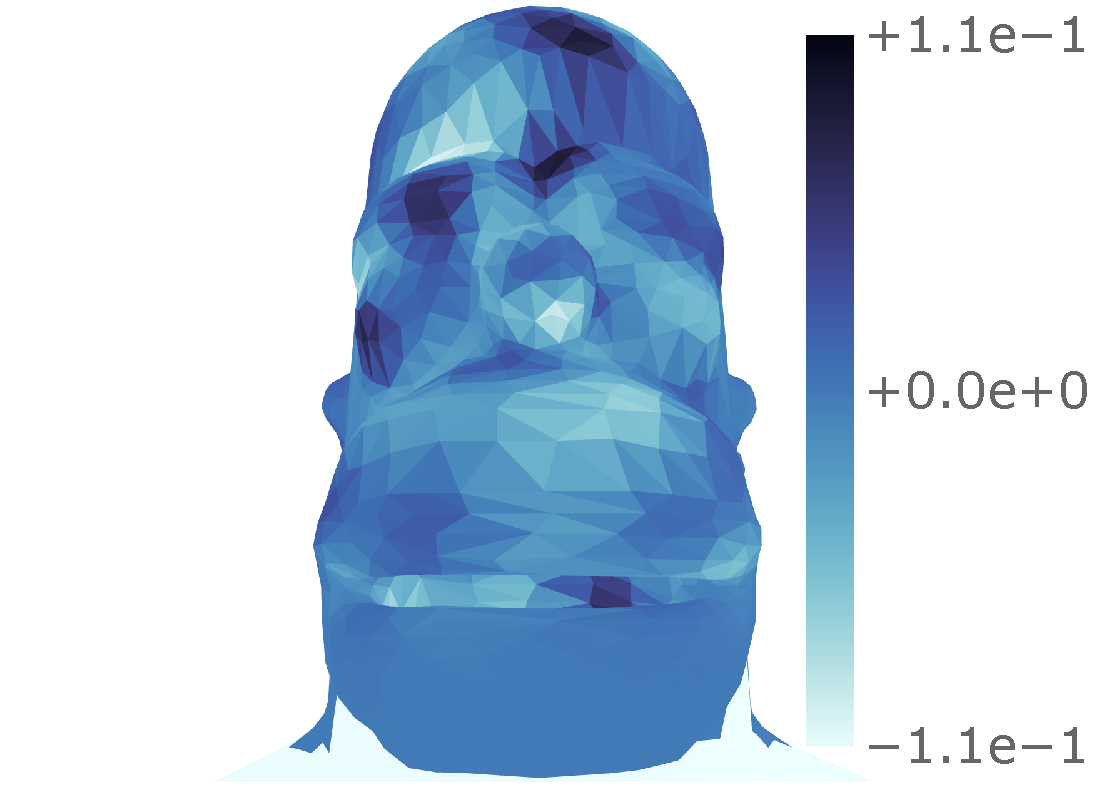
\includegraphics[trim={101 0 3 3},clip,width=.33\textwidth]{slepian_homer_rank49_lam1-000000e00_zoom.pdf}} % chktex 8
	\hfill
	\subfloat[\(\mesh{S_{100}},\ \mu_{100}=1.00\)]
	{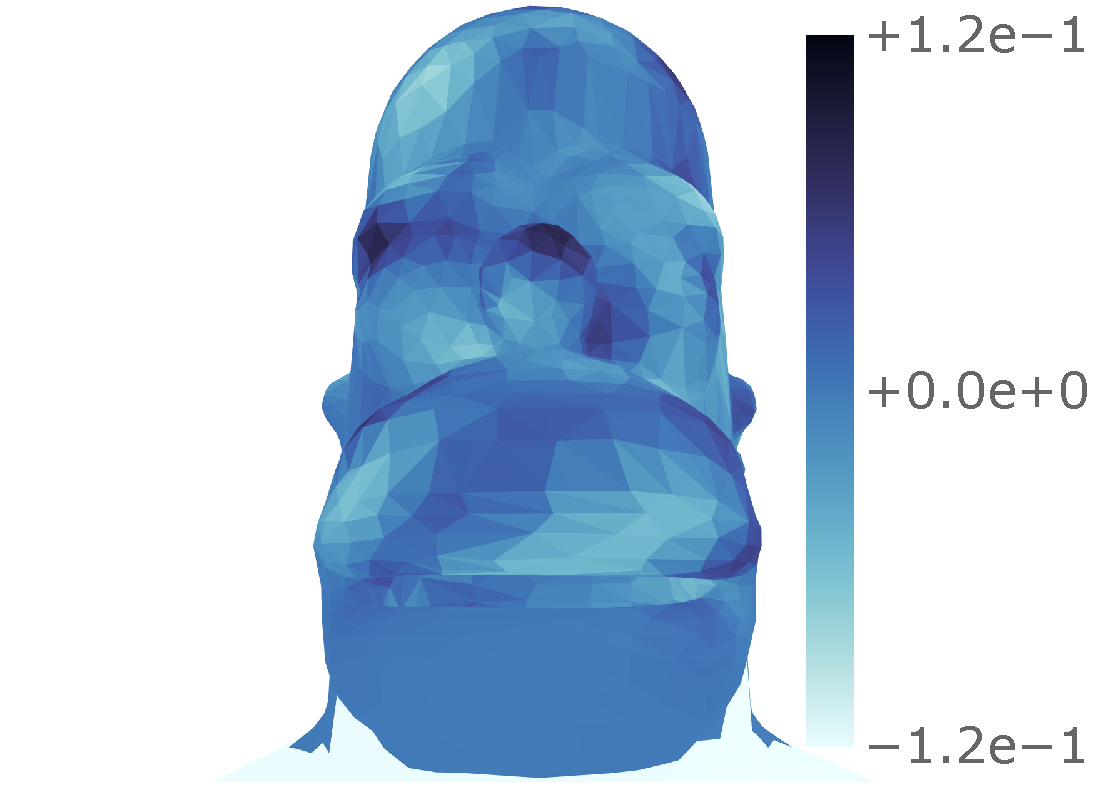
\includegraphics[trim={101 0 3 3},clip,width=.33\textwidth]{slepian_homer_rank99_lam1-000000e00_zoom.pdf}} % chktex 8
	\hfill
	\subfloat[\(\mesh{S_{200}},\ \mu_{200}=1.00\)]
	{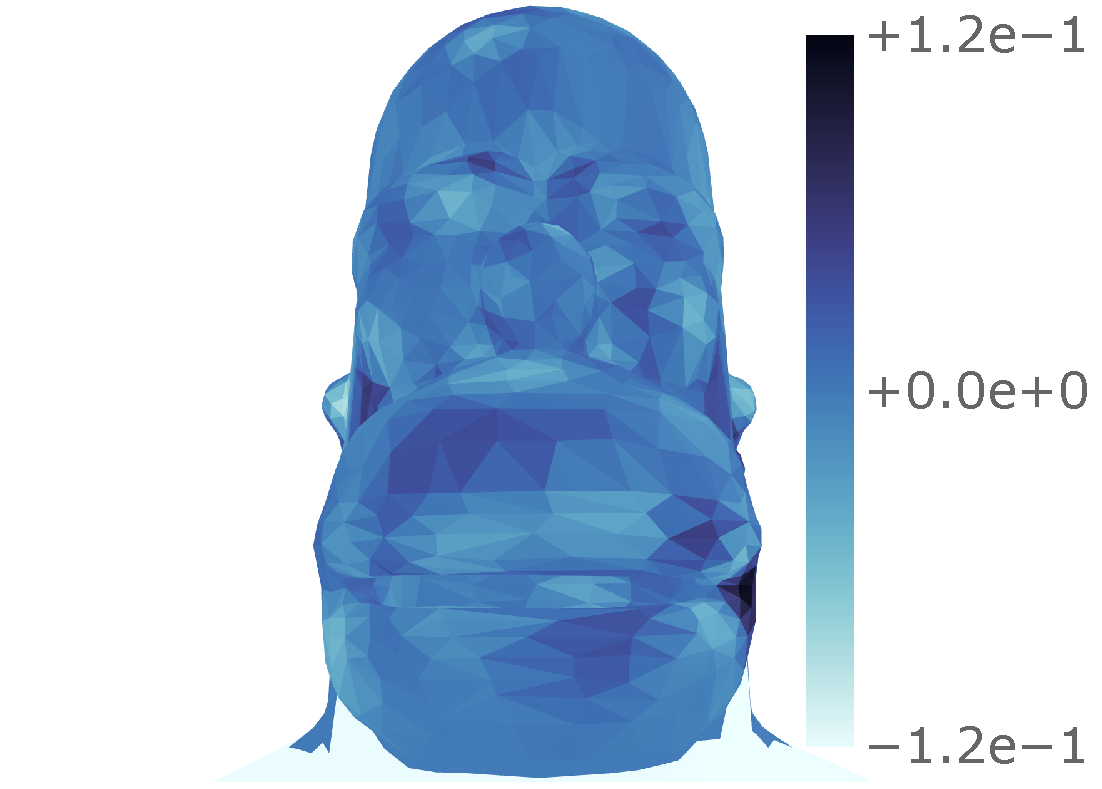
\includegraphics[trim={101 0 3 3},clip,width=.33\textwidth]{slepian_homer_rank199_lam1-000000e00_zoom.pdf}} % chktex 8
	\caption[
		Some Slepian functions of the Homer head region
	]{
		The Slepian functions of the Homer head region \(\mesh{\slepian{S}}\) for \(p \in \set{1, 10, 25, 50, 100, 200}\) shown left-to-right, top-to-bottom.
		The corresponding eigenvalue \(\slepian{\mu}\) is a measure of the concentration within the given region \(R\), that remains \(\almost{1}\) for many \(p\) values before decreasing towards zero.
		Whilst the Slepian functions are defined on the vertices, the values have been averaged onto the faces for the plot.
	}\label{fig:chapter5_slepian_functions}
\end{figure}
